\documentclass[11pt,a4paper]{article}
\usepackage[utf8]{inputenc}
\usepackage[T1]{fontenc}
\usepackage[spanish,es-noquoting]{babel}
\usepackage{lmodern,geometry,microtype}
\usepackage{amsmath,amssymb,amsthm,mathtools}
\usepackage{xcolor,booktabs,longtable,array}
\usepackage{hyperref,fancyhdr,graphicx,enumitem}
\geometry{top=24mm,bottom=25mm,left=25mm,right=25mm,headheight=15pt}
\hypersetup{colorlinks=true,linkcolor=blue!45!black,urlcolor=blue!45!black,pdftitle={O93 - Cierre propio, flujo y regularidad condicional}}
\pagestyle{fancy}\fancyhf{}\lhead{Programa de Geometría Relacional}\rhead{O93 · Suplemento de auditoría}\cfoot{\thepage}
\setlist[itemize]{leftmargin=1.4em,itemsep=2pt}\setlist[enumerate]{leftmargin=1.6em,itemsep=3pt}
\newtheorem{teo}{Teorema}[section]
\newtheorem{lem}[teo]{Lema}
\newtheorem{cor}[teo]{Corolario}
\theoremstyle{definition}\newtheorem{defi}[teo]{Definición}
\newcommand{\RR}{\mathbb{R}}\newcommand{\TT}{\mathbb{T}}
\newcommand{\mean}[1]{\langle #1\rangle}\newcommand{\pplus}[1]{\left[#1\right]_+}
\newcommand{\stat}[1]{\textcolor{blue!50!black}{\textsf{[#1]}}}
\title{\vspace{-1.3em}\textbf{O93 --- Cierre propio, doble normalización y regularidad condicional}\\[0.35em]
\large Reconstrucción formal y auditoría reproducible de Navier--Stokes desde la geometría relacional}
\author{\textbf{Programa de Geometría Relacional}\\Autoría del programa: \emph{Le Matt Ansatz Di Ego}\\Formalización integrada y verificaciones computacionales}
\date{22 de octubre de 2026 · Suplemento propuesto para la Imagen Total}
\begin{document}\maketitle
\begin{abstract}
Se reconstruye la transición ontológica del tetraedro relacional al circuito plano de cuatro cápsulas y se separan sus contratos cinemáticos del fluido físico. Se cotejan las formulaciones O72, O74--O75, O78, O80--O86, O88 y O92. Como resultado técnico integrador, las coordenadas de amplitud global y armónicos normalizados de O92 se conectan \emph{exactamente} al balance de enstrofía de O86: $W=M^2D$, $B=M^2D_2$, $P=M^3\mathcal T$. De ello se obtiene una reformulación equivalente de un criterio \emph{condicional} de continuación suave. Se adjuntan verificaciones simbólicas de la fase, la paridad del circuito y la actualización O84, además de soluciones exactas y una integración Fourier--Galerkin 3D con controles de malla y paso temporal. \textbf{No se demuestra la regularidad global para todos los datos 3D de Navier--Stokes, ni que cuatro cápsulas sean un mínimo físico universal.}
\end{abstract}
\tableofcontents\bigskip

\section{Reglas de lectura y procedencia}
La jerarquía del programa se conserva estrictamente: \emph{ontología y secuencia de lenguaje} $\rightarrow$ \emph{definiciones y matemáticas} $\rightarrow$ \emph{experimentos computacionales} $\rightarrow$ \emph{interpretación física sometida a contraste}. Las etiquetas son: \stat{O}, proposición ontológica; \stat{T}, demostración bajo hipótesis declaradas; \stat{E}, cálculo reproducible; \stat{F}, contraejemplo contra una afirmación delimitada; \stat{A}, puente abierto. El presente documento es \emph{aditivo}, no sustituye las pruebas ni los datos originales de O72--O92. Su reproducción certifica las comprobaciones especificadas, no una auditoría completa de todas las conversaciones antiguas.

\section{Capa ontológica: identidad sin figura obligatoria}
\paragraph{Secuencia narrativa \stat{O}.} Unidad sin diferencia acreditada; reflexión interna; comparación parte/todo; referencia normalizadora; resto o relación todavía no habitada; cierre propio; nueva circunstancia; transporte de la referencia que permite reconstruir lo común. La singularidad ontológica es un \emph{cierre propio que se sostiene}, no un punto físico infinito ni el \emph{blow-up} de una ecuación diferencial. Una configuración puede variar de forma, portadores materiales, radio y fase sin que la continuidad de la referencia se pierda por definición; que esto ocurra físicamente debe comprobarse.

\paragraph{Del tetraedro al circuito plano.} En el modelo abstracto $K_4$ hay cuatro nodos y seis enlaces activos. Al seleccionar solo los cuatro enlaces periféricos $C_4$, quedan dos diagonales no activas. \textbf{Proyectar la imagen 3D a un plano no elimina automáticamente las diagonales}; la selección de restricciones es una operación distinta. El circuito admite deformaciones internas y un modo cinemático alternado que un tetraedro completamente restringido no admite bajo las mismas leyes de enlaces. Desde una orientación de recorrido del plano aparece una normal con dos signos; su elección física requiere circulación y dinámica, no nace del dibujo. La palabra ``líquido'' es una \emph{hipótesis de realización} de estas libertades, no una consecuencia lógica de ser $C_4$.

\paragraph{Realizaciones del cierre.} Anillo, esfera y ola/onda son contratos distintos de reconocimiento, no tres formas obligatorias de un solo objeto físico. Un patrón ondulatorio puede ser reconocible aun cambiando sus portadores y amplitud, pero periodicidad de fase no equivale a estado idéntico, ni onda viscosa de cizalla a solitón de superficie. Los dos giros del anillo son fases poloidal y toroidal; sus marcas móviles no deben confundirse con partículas privilegiadas.

\section{Capa matemática I: circuito, paridad y holonomía}
\begin{defi}[Grafo de enlaces exteriores]
Sea $G=(V,E)$ conectado, con $n$ vértices y velocidades tangenciales firmadas $s_i$. Cada enlace exterior ideal impone $s_i+s_j=0$. La matriz $Q_G$ tiene dos unos por cada fila y $Q_Gs=0$.
\end{defi}
\begin{teo}[Paridad de enlaces, O72 \stat{T}]
Si $G$ es bipartito, $\dim\ker Q_G=1$; si contiene un ciclo impar, $\dim\ker Q_G=0$. Para $C_4$ se tiene $s=(a,-a,a,-a)$, con $a\in\RR$; para el triángulo $C_3$ y el tetraedro completo $K_4$ solo existe $s=0$.
\end{teo}
\begin{proof}
Partiendo de un vértice, la condición del enlace obliga a alternar el signo al atravesar una arista. En un grafo bipartito toda trayectoria mantiene una asignación consistente, determinada por un único escalar $a$. Si existe ciclo impar, al regresar al origen se obtiene $a=-a$, luego $a=0$ y la conexión fuerza todos los demás a cero. En $C_4$ las cuatro ecuaciones se satisfacen con el vector indicado. El verificador E1 calcula las matrices y rangos exactos.
\end{proof}
Para un cuadrilátero genérico articulado en el plano: $8$ coordenadas menos $3$ movimientos rígidos menos $4$ longitudes periféricas independientes deja \textbf{una libertad geométrica}. No es la misma que el escalar $a$ de velocidad. Un tetraedro genérico con seis distancias rígidas no conserva esta flexión interna. Estos conteos dependen de la genericidad y la elección de enlaces.

\begin{teo}[Compatibilidad de cuatro contactos, O74 \stat{T}]
Para brazos de contacto positivos $a_i,b_i$ y enlaces $a_i\omega_i+b_i\omega_{i+1}=0$ con índices módulo $4$, existe un modo no nulo si y solo si
\begin{equation}\label{eq:H}H=\prod_{i=1}^{4}\frac{a_i}{b_i}=1.\end{equation}
Si $a_i=r_i$, $b_i=r_{i+1}$, entonces $H=1$ para cualesquiera $r_i>0$.
\end{teo}
\begin{proof}
Componer las cuatro ecuaciones da $\omega_5=H\omega_1$; el cierre exige $\omega_5=\omega_1$. Para $\omega_1\ne0$ equivale a $H=1$. Con brazos consecutivos idénticos en cada nodo el producto telescopa: $(r_1/r_2)(r_2/r_3)(r_3/r_4)(r_4/r_1)=1$.
\end{proof}
\noindent\textbf{Alcance:} la holonomía $H=1$ \emph{no} acota las frecuencias, garantiza forma no degenerada, fuerza fases periódicas comunes ni representa una ley impuesta por Navier--Stokes. O75 deriva una \emph{holonomía de deformación material} $H_F$ diferente, con $\frac{d}{dt}\log H_F$ expresable por diferencias de estiramientos locales; soluciones exactas de NS pueden hacerla variar. La incompresibilidad material $\det D\Phi_t=1$ tampoco obliga a conservar ángulos rectos.

\section{Capa matemática II: dos giros y reconstrucción de fases}
En un toro geométrico con fases $\theta$ (tubo/poloidal) y $\varphi$ (aro/toroidal), sean $p,q$ coprimos, y defínase $\Psi=p\theta-q\varphi$. Bajo $\dot\theta=q\Omega(t)$ y $\dot\varphi=p\Omega(t)$ se deduce $\dot\Psi=0$. Esto es un \emph{modelo cinemático}, no una condición universal de NS. El entero de repetición y el retorno material son afirmaciones distintas.

Por Bézout, existen $b,c\in\mathbb Z$ con $bq+cp=1$. La transformación
\begin{equation}
\begin{pmatrix}\Phi\\\Psi\end{pmatrix}=
\begin{pmatrix}b&c\\p&-q\end{pmatrix}
\begin{pmatrix}\theta\\\varphi\end{pmatrix},\qquad \det=-1,
\end{equation}
es unimodular e invertible en el toro de fases (O68/O88). Si luego se multiplican fases por $N>1$, la aplicación pierde unicidad de preimagen: hay que conservar además la etiqueta de rama. Esta operación formaliza \emph{reconstruibilidad de representación}; no determina por sí sola un límite a la vorticidad.

\section{Capa matemática III: doble normalización en Navier--Stokes}
\subsection{Contrato físico y notación}
Trabajamos en el toro periódico $\TT^3=(\RR/2\pi\mathbb Z)^3$, con $\nu>0$, sin fuerza, campo $u(x,t)$ suave, real, solenoidal y de media cero en el intervalo de existencia. La presión se normaliza por densidad. Se usa promedio espacial $\mean{\cdot}$ y coeficientes Fourier de Parseval con $\mean{|u|^2}=\sum_k|\widehat u_k|^2$.
\begin{equation}\label{eq:NS}
\partial_tu+(u\cdot\nabla)u=-\nabla p+\nu\Delta u,\qquad \nabla\cdot u=0,\qquad \omega=\nabla\times u.
\end{equation}
\begin{defi}[Coordenadas normalizadas de O92]
Sea $M>0$ la magnitud global del campo y $z_k$ sus componentes complejas normalizadas:
\begin{equation}\label{eq:coords}
M=\left(\sum_{k\ne0}|\widehat u_k|^2\right)^{1/2},\quad
z_k=\widehat u_k/M,\quad \sum_{k\ne0}|z_k|^2=1.
\end{equation}
Se conservan fases y polarizaciones vectoriales (no solo $|z_k|$). Póngase
\begin{gather}
D=\sum_{k\ne0}|k|^2|z_k|^2,\qquad D_2=\sum_{k\ne0}|k|^4|z_k|^2,\\
\mathcal B_k(z,z)=-i\mathbb P_k\sum_{p+q=k}(q\cdot z_p)z_q,
\quad \mathbb P_k=I-\frac{kk^\top}{|k|^2},\\
\mathcal T=\sum_{k\ne0}|k|^2\operatorname{Re}\big(\overline{z_k}\cdot\mathcal B_k(z,z)\big).
\end{gather}
\end{defi}
\begin{teo}[Dinámica exacta en coordenadas normalizadas, O92 \stat{T}]
En todo intervalo suave con $M>0$,
\begin{equation}\label{eq:o92}
\boxed{\dot M=-\nu MD,\qquad
\dot z_k=-\nu(|k|^2-D)z_k+M\mathcal B_k(z,z).}
\end{equation}
Además,
\begin{equation}\label{eq:D}
\boxed{\dot D=-2\nu(D_2-D^2)+2M\mathcal T.}
\end{equation}
\end{teo}
\begin{proof}
La ecuación Fourier proyectada es $\dot{\widehat u}_k=-\nu|k|^2\widehat u_k+M^2\mathcal B_k(z,z)$. La cancelación de transporte en el balance cinético da $\frac{d}{dt}M^2=-2\nu M^2D$ y por tanto la primera ecuación. Diferenciar $z_k=\widehat u_k/M$ produce la segunda. Derivar $D=\sum|k|^2|z_k|^2$, usar la segunda ecuación y separar los términos viscosa y no lineal prueba \eqref{eq:D}. Se requiere conservar la colección completa de coeficientes: \emph{no} es una compresión a dimensión finita.
\end{proof}
\subsection{El puente exacto O92 $\leftrightarrow$ O86}
Definimos enstrofía, palinstrofía y estiramiento con el \emph{mismo} convenio de promedio espacial:
\begin{equation}
W=\mean{|\omega|^2},\qquad B=\mean{|\nabla\omega|^2},\qquad
P=\mean{\omega\cdot S\omega},\quad S=\tfrac12(\nabla u+\nabla u^\top).
\end{equation}
\begin{teo}[Correspondencia exacta de los balances \stat{T}]\label{th:puente}
Para soluciones del contrato anterior, en tiempos suaves,
\begin{equation}\label{eq:puente}
\boxed{W=M^2D,\qquad B=M^2D_2,\qquad P=M^3\mathcal T.}
\end{equation}
En consecuencia,
\begin{equation}\label{eq:balance}
\boxed{\frac12\frac{d}{dt}(M^2D)=M^3\mathcal T-\nu M^2D_2=P-\nu B.}
\end{equation}
\end{teo}
\begin{proof}
Para campo solenoidal $k\cdot\widehat u_k=0$, la identidad $|k\times\widehat u_k|^2=|k|^2|\widehat u_k|^2$ y Parseval dan $W=\sum|k|^2|\widehat u_k|^2=M^2D$ y $B=\sum|k|^4|\widehat u_k|^2=M^2D_2$. Derivar $M^2D$ usando \eqref{eq:o92}--\eqref{eq:D} resulta $\frac12W'=M^3\mathcal T-\nu M^2D_2$. Por el balance exacto de vorticidad $\frac12W'=P-\nu B$ de O39/O86, y sustituyendo $B=M^2D_2$, se identifica $P=M^3\mathcal T$.
\end{proof}
\noindent\textbf{Importancia y límite.} La transferencia triádica normalizada y el estiramiento físico se representan por la misma cantidad. La identidad \emph{no} impone signo ni acotación universal a $\mathcal T$; es una reexpresión fiel de NS.

\section{Capa matemática IV: un criterio condicional de regularidad}
Defínanse el radio espectral endógeno de O25/O86, su reloj viscoso y el cociente de compensación:
\begin{equation}\label{eq:reloj}
\ell_\omega^2=\frac WB=\frac D{D_2},\quad
d\tau_\nu=\frac{\nu B}{W}\,dt=\nu\frac{D_2}{D}\,dt,\quad
\Gamma_\nu=\frac{P}{\nu B}=\frac{M\mathcal T}{\nu D_2}.
\end{equation}
\begin{teo}[Criterio de continuación en doble normalización \stat{T/C}]\label{th:criterion}
Sea $u$ solución clásica en $[0,T_*)$, $0<T_*<\infty$, dato inicial suave, de media cero y no nulo; supóngase $\nu>0$ y las cantidades \eqref{eq:reloj} definidas en el intervalo. Si
\begin{equation}\label{eq:criterio}
\boxed{\int_0^{T_*}\frac{\pplus{M(t)\mathcal T(t)-\nu D_2(t)}}{D(t)}\,dt<\infty,}
\end{equation}
entonces $\sup_{t<T_*}W(t)<\infty$ y la solución se prolonga suavemente más allá de $T_*$ por los criterios clásicos de continuación de datos suaves periódicos.
\end{teo}
\begin{proof}
De \eqref{eq:balance} y \eqref{eq:reloj} se obtiene
$\frac{d}{d\tau_\nu}\log W=2(\Gamma_\nu-1)$. Integrar da
\[W(t)=W(0)\exp\left[2\int_0^{\tau_\nu(t)}(\Gamma_\nu-1)\,d\tau_\nu\right].\]
Además, por $D,D_2,\nu>0$,
\[
\pplus{\Gamma_\nu-1}\,d\tau_\nu
=\frac{\pplus{M\mathcal T-\nu D_2}}{D}\,dt.
\]
La integral del lado derecho acotada uniformemente antes de $T_*$ acota $W(t)$ mediante la fórmula exponencial; la energía cinética $M^2$ es no creciente. Así se conserva una cota $H^1$ en un dominio periódico, suficiente para el criterio estándar de continuación de soluciones fuertes suaves de NS 3D.
\end{proof}
\begin{cor}[Lo que permanece abierto \stat{A}]
La identidad de este criterio no demuestra que \eqref{eq:criterio} se cumpla para \emph{todos} los datos iniciales suaves tridimensionales. Haría falta obtener la finitud de esa integral \emph{a priori} de NS o de una ley física adicional probada, sin escoger referencias después de conocer el futuro.
\end{cor}

\section{Otra vía demostrada: referencias y defecto actualizado (O82--O84)}
Para una referencia física computable $U_j(t)$, escribimos $u=U_j+v_j$, $N(f,g)=\mathbb P\nabla\cdot(f\otimes g)$ y $N(u)=N(u,u)$. En el intervalo $I_j=[t_j,t_{j+1})$:
\begin{equation}
F_j=\partial_tU_j+N(U_j)-\nu\Delta U_j,\quad
R(f)=\sum_{k\ne0}\frac{|\widehat f_k|}{|k|},\quad
S(f)=\sum_{k\ne0}|\widehat f_k|,\quad
Q(f)=\sum_{k\ne0}|k|\,|\widehat f_k|.
\end{equation}
Se preserva la hipótesis de presupuesto local de O82/O84
\begin{equation}\label{eq:defecto}
D^+R(v_j)+\frac\nu4Q(v_j)\le g_jR(v_j)+R(F_j),\qquad g_j=\frac4\nu S(U_j)^2,
\end{equation}
\emph{en el régimen bootstrap} $R(v_j)\le\nu/2$. Esta desigualdad fue derivada en la rama anterior; aquí se reproduce su consecuencia de contabilidad y se explicitan sus supuestos.

\begin{lem}[Contabilidad sin volver a cobrar el resto, O84 \stat{T}]
Defínanse $G(t)=\int_0^tg_{j(s)}(s)ds$, los saltos de referencia $J_j=R(U_{j-1}(t_j)-U_j(t_j))$ y
\[
\mathcal C(t)=R(v_0)+\int_0^te^{-G(s)}R(F_{j(s)}(s))ds
+\sum_{0<t_j\le t}e^{-G(t_j)}J_j.
\]
Siempre que las cotas anteriores apliquen en los intervalos,
\begin{equation}\label{eq:conta}
\boxed{e^{-G(t)}R(v(t))+\frac\nu4\int_0^te^{-G(s)}Q(v(s))ds\le\mathcal C(t).}
\end{equation}
\end{lem}
\begin{proof}
Multiplicar \eqref{eq:defecto} por $e^{-G(t)}$ e integrar en cada intervalo. Los términos de frontera del resto se cancelan entre intervalos contiguos. El único costo adicional permitido por desigualdad triangular es el salto $J_j$; sumarlo una vez, con su peso, produce \eqref{eq:conta}. Para infinitos intervalos se requiere convergencia de los costos positivos para efectuar el límite.
\end{proof}
\noindent Si $G_*<\infty$, $e^{G_*}\mathcal C_*<\nu/2$ y $\sum_j\int_{I_j}Q(U_j)dt<\infty$ en un horizonte finito, O84 da la integral temporal finita de $\|\nabla u\|_\infty$ y continuación suave. Son \emph{hipótesis efectivas}, no restricciones que NS garantice universalmente.

\paragraph{Actualización sin salto.} Defínase $C(t)=-\int_a^t e^{\nu(t-s)\Delta}F_U(s)ds$ y $U^+=U+C$. Entonces $C(a)=0$, no se introduce costo de salto y
\[
F_{U^+}=N(U,C)+N(C,U)+N(C,C).
\]
Esta identidad incorpora interacciones que no estaban presentes en la primera referencia; no asegura por sí sola convergencia tras infinitas iteraciones.

\section{Laboratorios y resultados efectivamente ejecutados}
Los programas adjuntos son archivos nuevos, no una presentación como si fueran los códigos originales O72--O92. El verificador exacto usa \texttt{SymPy}, \texttt{mpmath} y \texttt{NumPy}. La integración adicional usa Fourier--Galerkin 3D, de-aliasing $2/3$, proyección de Leray y RK4; se comparan dos mallas y dos pasos de tiempo. El código conserva los datos iniciales y todas las convenciones de normalización.

\subsection*{E1--E2. Paridad y holonomía \stat{E}}
Matrices exactas dan $\dim\ker Q_{C_3}=0$, $\dim\ker Q_{C_4}=1$ y $\dim\ker Q_{K_4}=0$. Productos de radios positivos que se telescopan dan $H=1$, mientras una asimetría no compensada de $10\%$ da $H=1.1$. Son comprobaciones de las proposiciones bajo la regla ideal, no fluidos simulados.

\subsection*{E3. Dos fases con las mismas magnitudes y efectos distintos \stat{T/E/F}}
La familia de O86 toma los vectores de onda $k=(1,0,0)$, $l=(0,1,1)$, $m=k+l=(1,1,1)$, $h=(0,0,1)$ y el campo
\begin{align}
u_0(x,y,z)={}&(0,1,0)\cos x+(1,0,0)\cos(y+z)\\
&+c(1,1,-2)\sin(x+y+z)+\tfrac13(1,0,0)\cos z,
\qquad c\in\{-1,+1\}.
\end{align}
La suma Fourier con coeficientes racionales e imaginarios exactos, sin cuadratura ni truncación temporal, verifica:
\begin{equation}\label{eq:phaseresult}
\boxed{W(0)=\frac{95}{9},\quad B(0)=\frac{266}{9},\quad P(0)=\frac{3c}{4}.}
\end{equation}
Para $\nu=1/100$,
\begin{equation}
\Gamma_\nu(0)=c\frac{675}{266},\qquad
\dot W(0)=\begin{cases}409/450& c=+1,\\ -941/450&c=-1.\end{cases}
\end{equation}
Los dos estados tienen los mismos pesos Fourier y la misma escala $W/B$, pero la orientación/fase cambia el estiramiento. \textbf{Refuta que amplitudes y radio espectral basten por sí solos para predecir esa transferencia}; no implica explosión de una solución.

\subsection*{E4. Ondas de cizalla exactas \stat{T/E}}
Para $u=(\sum_{j=1}^{4}a_j e^{-\nu k_j^2 t}\sin(k_j y),0,0)$, con $k_j=1,2,3,4$ y $\nu=0.12$, el término convectivo se anula exactamente: es una solución de NS para todo $t\ge0$. El verificador compara para $51$ tiempos las identidades de O92 y la ley de varianza de O78; $\mathcal T=0$, $D'=-2\nu(D_2-D^2)\le0$. No debe confundirse esta onda de campo de velocidad con un solitón superficial.

\subsection*{E5. Actualización y certificado O84 \stat{T/E}}
Para $u_0=(4\sin y,\sin z,\sin x)$, $\nu=1$ y $\delta=9/500$, se reproducen con $65$ dígitos:
\[
\mathfrak M_0=0.519488712836\ldots>\tfrac12,\qquad
\mathfrak M_1\le0.271724746561\ldots<\tfrac12.
\]
La primera referencia no pasa el criterio suficiente en ese intervalo; la referencia actualizada sí. El verificador evalúa fórmulas analíticas del documento O84, no integra la trayectoria exacta y no demuestra regularidad universal.

\subsection*{E6. Fourier--Galerkin 3D independiente \stat{E}}
Los datos de E3 se integraron con $\nu=0.01$ hasta $T=0.08$. La tabla muestra $W(T)$ del modelo truncado:
\begin{center}\begin{tabular}{lrr}\toprule
Esquema & Fase $c=+1$ & Fase $c=-1$\\\midrule
$N=16$, $\Delta t=0.004$ & 10.661906020719 & 10.423743782495\\
$N=24$, $\Delta t=0.004$ & 10.661906020720 & 10.423743782496\\
$N=24$, $\Delta t=0.002$ & 10.661906020726 & 10.423743782501\\\bottomrule
\end{tabular}\end{center}
Las diferencias de resolución y paso temporal son cercanas a $10^{-12}$ para este experimento corto. No se extrapolan a tiempos largos ni a límites de regularidad. En $t=0$ ambas preparaciones satisfacen \eqref{eq:phaseresult} hasta error de redondeo.
\begin{center}\IfFileExists{figuras/galerkin_fases.png}{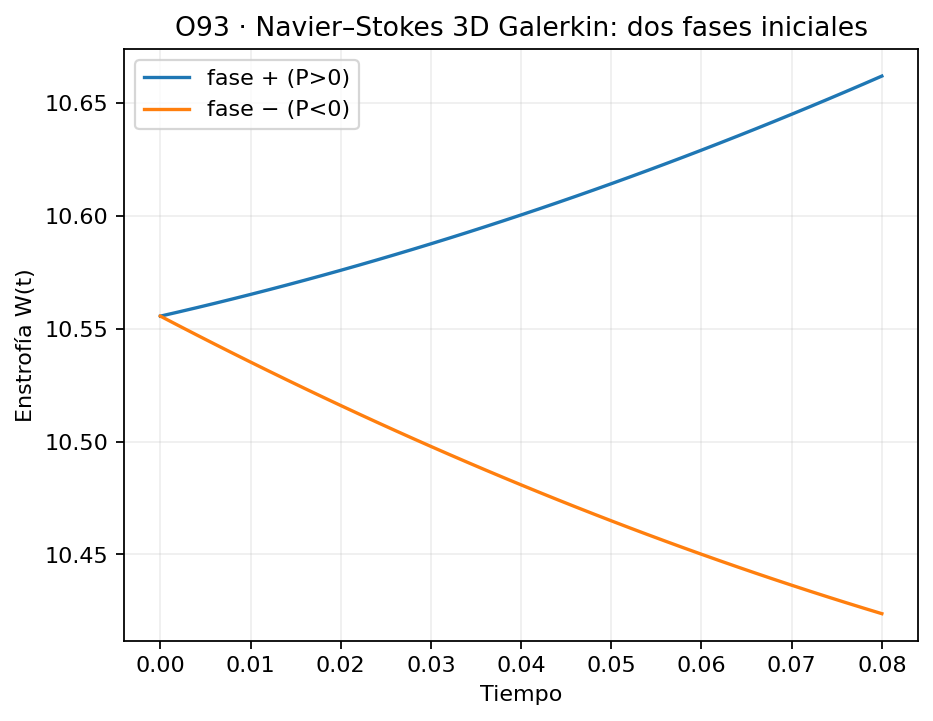
\includegraphics[width=.78\linewidth]{figuras/galerkin_fases.png}}{}\end{center}

\section{Matriz de afirmaciones y falsadores}
\small
\begin{longtable}{p{0.51\textwidth}p{0.12\textwidth}p{0.26\textwidth}}
\toprule Afirmación precisa & Estado & Condición / evidencia\\\midrule\endfirsthead
\toprule Afirmación precisa & Estado & Condición / evidencia\\\midrule\endhead
$C_4$ admite modo alternado no nulo, $K_4$ no & \stat{T/E} & Grafo de contactos ideales (O72, E1)\\
$H=1$ permite giros compatibles con radios variables & \stat{T/E} & Contactos ideales (O74, E2)\\
La forma anular obliga a una dirección física de avance & \stat{A} & Requiere dinámica y circulación independientes\\
Un cierre de cuatro nodos es conservación universal en NS & \stat{F} & O75 proporciona contraejemplos\\
Fase cambia estiramiento aunque coincidan $W,B$ & \stat{T/E} & Campo trigonométrico O86, E3--E6\\
$W=M^2D$, $B=M^2D_2$, $P=M^3\mathcal T$ & \stat{T} & Solución suave, Fourier completo\\
Finitud de \eqref{eq:criterio} implica continuación suave & \stat{T/C} & Criterio suficiente en $\TT^3$\\
La finitud de \eqref{eq:criterio} vale para todo dato suave 3D & \stat{A} & No demostrado\\
O84 permite actualizar referencias sin doble contabilizar & \stat{T/E} & Presupuestos bajo bootstrap y defectos\\
La doble normalización conserva información sin infinitos modos & \stat{F/A} & Solo reconstrucción con todos los $z_k$; compresión no probada\\
El programa resolvió el problema Clay de NS 3D general & \stat{No} & No se dispone de prueba universal\\
\bottomrule
\end{longtable}\normalsize

\section{Obligación de prueba para una conexión generativa universal}
Sea $C_j$ una referencia producida por una regla explícita \emph{a partir de datos iniciales y actualización causal}, sin usar la solución futura como oráculo. Demostrar un principio físico nuevo requeriría, conjuntamente:
\begin{enumerate}
\item \textbf{Cobertura:} definir nodos, fases y referencias para todos los datos iniciales de la clase buscada o una clase amplia explícita; no presuponer anillos.
\item \textbf{Compatibilidad dinámica:} probar que $C_{j+1}$ reconstruye las relaciones relevantes de $C_j$ y que el defecto se controla bajo la evolución NS, incluyendo presión y triadas de fase.
\item \textbf{Presupuesto a priori:} derivar para cada $T_*<\infty$ un control uniforme de \eqref{eq:criterio}, o del presupuesto O84, sin hipótesis que ya equivalgan a la regularidad buscada.
\item \textbf{Contraste adversarial:} superar los pares de fases O79/O86, la presión no local de O76 y el escalado de costos O85; registrar resultados negativos sin redefinir retrospectivamente la referencia.
\end{enumerate}
El estado actual permite expresar estos requisitos y demostrar teoremas para clases y presupuestos definidos; \emph{no} permite declarar que se cumplen universalmente.

\section{Instrucciones para reproducir y auditar}
Desde el directorio del paquete, en Python 3.10 o superior:
\begin{verbatim}
python -m pip install -r requirements.txt
python experimentos/verificar_o93.py
python experimentos/simulacion_galerkin.py
\end{verbatim}
Se generan archivos JSON y CSV en \texttt{experimentos/resultados}, además de una gráfica en \texttt{figuras}. El archivo \texttt{README.md} identifica cada salida, sus parámetros y sus límites. Un manifiesto SHA-256 permite comprobar la integridad de los archivos de trabajo.

\section{Proveniencia documental}
\begin{itemize}
\item \textbf{Ontología, proyección y circuito:} Núcleo Canónico; O40; O58; O72, O74, O75.
\item \textbf{Espejo y reloj:} O25 y O45; \textbf{anillo, doble giro y reconstrucción:} O68, O87, O88.
\item \textbf{Resultados físicos y limitaciones:} O73 (axisimétrico sin giro); O76 (presión no local); O78 (ondas exactas); O79 (fases); O80--O85 (presupuestos de continuación y actualizaciones).
\item \textbf{Puente matemático central:} O86 (enstrofía, compensación y reloj), O92 (doble normalización y transferencia triádica).
\end{itemize}
Los documentos anteriores no se atribuyen como nuevas demostraciones a O93. Sus pruebas y contraejemplos mantienen su ámbito propio. Este suplemento agrega el cotejo explícito entre O86 y O92, la reformulación \eqref{eq:criterio} y un conjunto independiente de verificaciones reproducibles.
\vfill\noindent\textit{Fin de suplemento. Su incorporación como versión canónica queda sujeta a revisión crítica del programa.}
\end{document}
